%\documentclass[draft,10pt]{beamer}
\documentclass[10pt]{beamer}
\usetheme[progressbar=frametitle]{metropolis}
\usepackage{graphicx}
\usepackage{appendixnumberbeamer}
\usepackage{booktabs}
\usepackage{multirow}% to make table
\usepackage[scale=2]{ccicons}
\usepackage{FiraSans}
\usepackage{pgfplots}
\usepgfplotslibrary{dateplot}
\usepackage{xspace}
\usepackage{animate}
\usepackage{subfigure}
\usepackage{tikz}
\usetikzlibrary{shapes,arrows,shapes.misc}

\title{Restoration of riparian vegetation in the Hunhe River basin, Liaoning, China}
\date{19.12.2018}
\author{Shuai Yu$^\dag$\\ Jinlei Zhu$^\ddag$}
\institute{$^\dag$Institute of Applied Ecology, Chinese Academy of Sciences\\
$^\ddag$Institute of Landscape and Plant Ecology, University of Hohenheim}

\begin{document}
	\graphicspath{{figures/}}
	\maketitle
	\begin{frame}[t]{Acknowledgements}
\begin{columns}[t,onlytextwidth]
	\column{0.495\textwidth}
	\begin{figure}
		\centering
		\frame{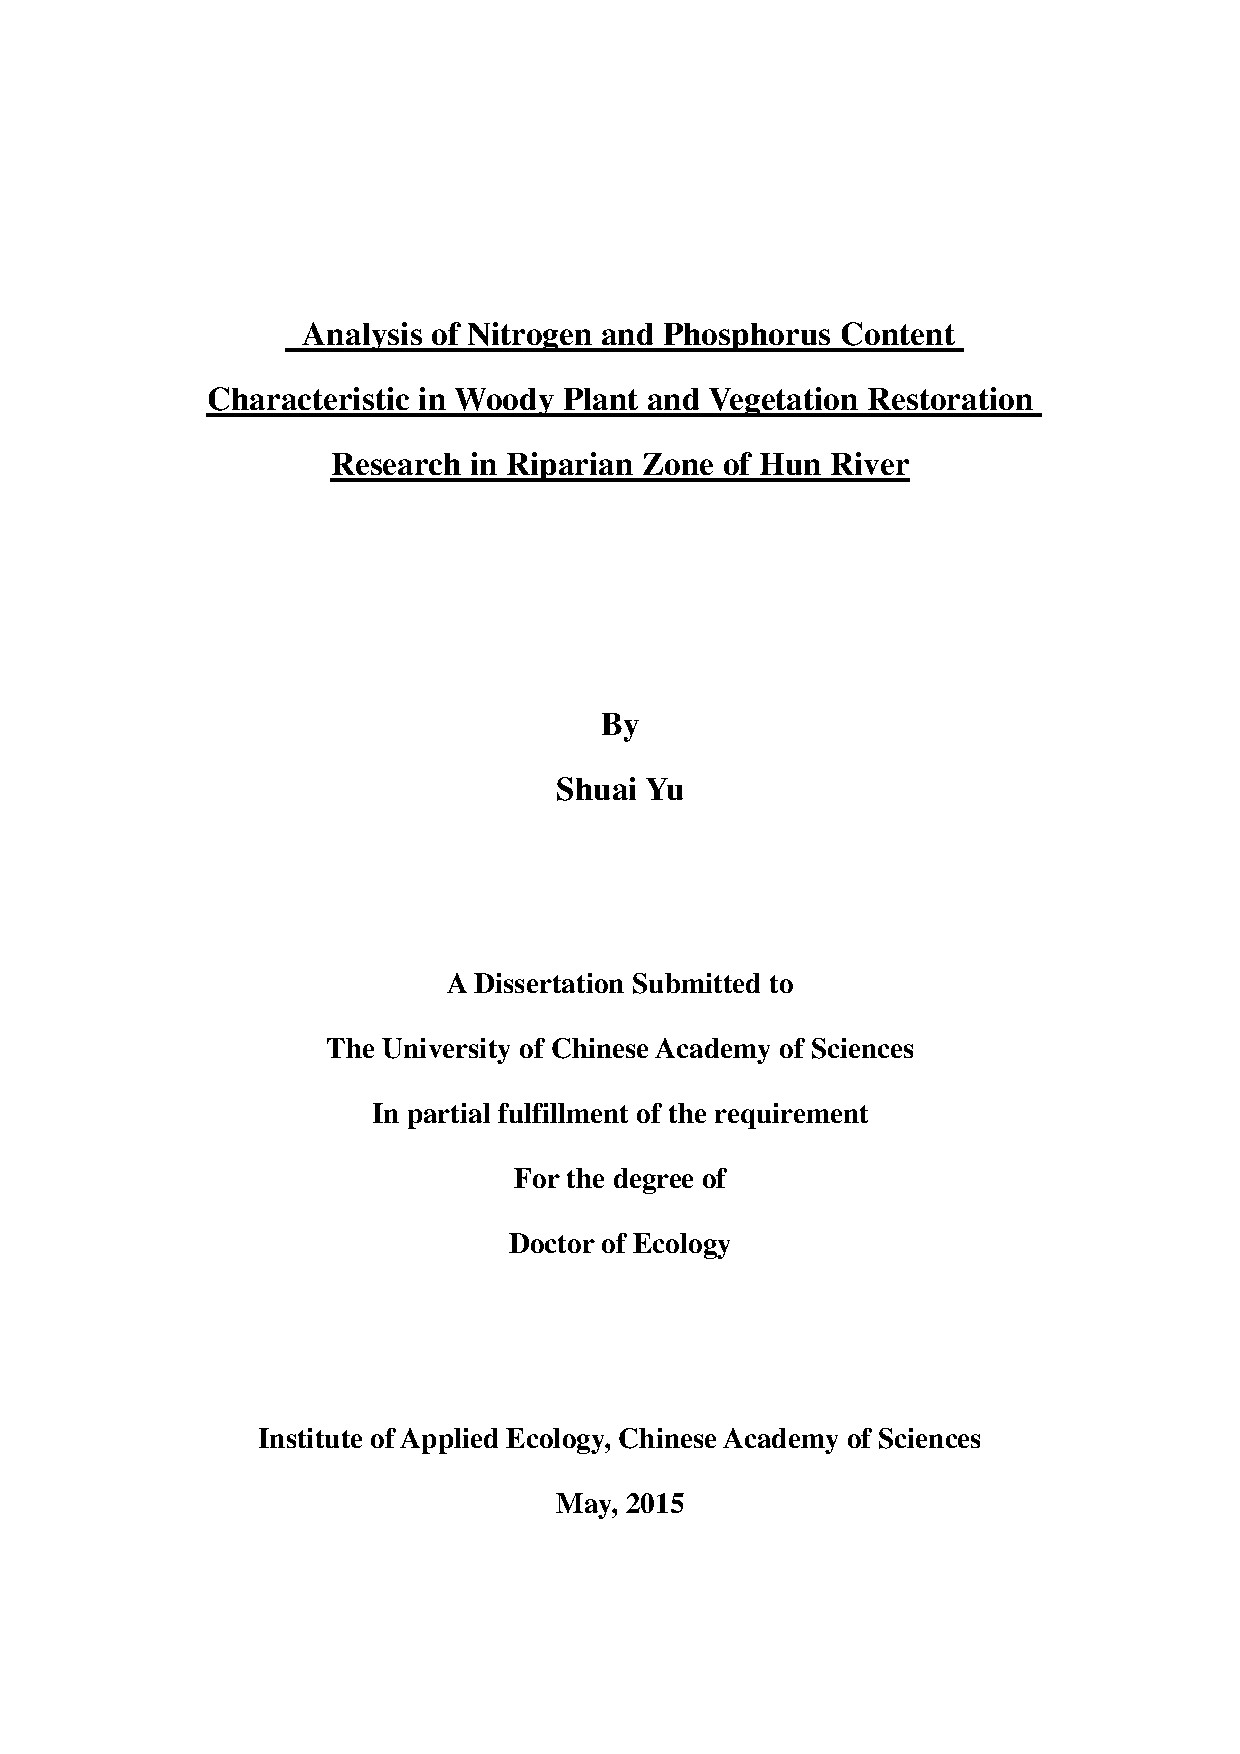
\includegraphics[width=\textwidth]{yushuaidissertationcover.pdf}}		
	\end{figure}
	\column{0.01\textwidth}
	\column{0.495\textwidth}
	\begin{figure}
		\centering
		\frame{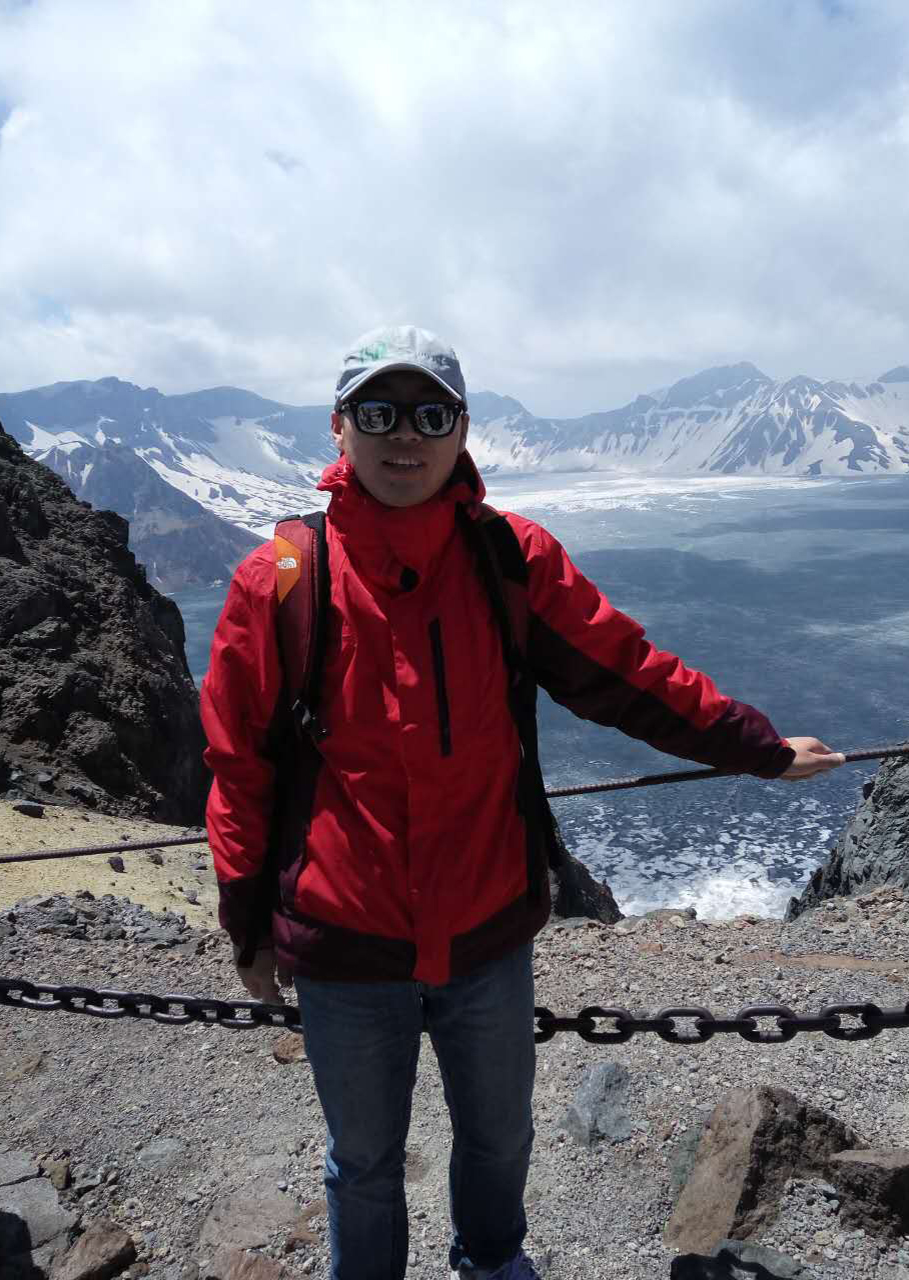
\includegraphics[width=\textwidth]{yushuaionchangbaishan.jpg}}
	\end{figure}	
\end{columns}
\end{frame}

	\section*{Outline}
\begin{frame}{Outline}
\setbeamertemplate{section in toc}[sections numbered]
\tableofcontents[hideallsubsections]
\end{frame}
	\section{Introduction}
\begin{frame}[fragile]{Metropolis}

  The \themename theme is a Beamer theme with minimal visual noise
  inspired by the \href{https://github.com/hsrmbeamertheme/hsrmbeamertheme}{\textsc{hsrm} Beamer
  Theme} by Benjamin Weiss.

  Enable the theme by loading

  \begin{verbatim}    \documentclass{beamer}
    \usetheme{metropolis}\end{verbatim}

  Note, that you have to have Mozilla's \emph{Fira Sans} font and XeTeX
  installed to enjoy this wonderful typography.
\end{frame}

\begin{frame}[fragile]{Sections}
  Sections group slides of the same topic

  \begin{verbatim}    \section{Elements}\end{verbatim}

  for which \themename provides a nice progress indicator \ldots
\end{frame}
	\section{Situation \& Problems}

\begin{frame}{Metropolis titleformats}
	\themename supports 4 different titleformats:
	\begin{itemize}
		\item Regular
		\item \textsc{Smallcaps}
		\item \textsc{allsmallcaps}
		\item ALLCAPS
	\end{itemize}
	They can either be set at once for every title type or individually.
\end{frame}

{
    \metroset{titleformat frame=smallcaps}
\begin{frame}{Small caps}
	This frame uses the \texttt{smallcaps} titleformat.

	\begin{alertblock}{Potential Problems}
		Be aware, that not every font supports small caps. If for example you typeset your presentation with pdfTeX and the Computer Modern Sans Serif font, every text in smallcaps will be typeset with the Computer Modern Serif font instead.
	\end{alertblock}
\end{frame}
}

{
\metroset{titleformat frame=allsmallcaps}
\begin{frame}{All small caps}
	This frame uses the \texttt{allsmallcaps} titleformat.

	\begin{alertblock}{Potential problems}
		As this titleformat also uses smallcaps you face the same problems as with the \texttt{smallcaps} titleformat. Additionally this format can cause some other problems. Please refer to the documentation if you consider using it.

		As a rule of thumb: Just use it for plaintext-only titles.
	\end{alertblock}
\end{frame}
}

{
\metroset{titleformat frame=allcaps}
\begin{frame}{All caps}
	This frame uses the \texttt{allcaps} titleformat.

	\begin{alertblock}{Potential Problems}
		This titleformat is not as problematic as the \texttt{allsmallcaps} format, but basically suffers from the same deficiencies. So please have a look at the documentation if you want to use it.
	\end{alertblock}
\end{frame}
}
	\section{Solutions}

%N, P accumulation ability
\begin{frame}{N, P accumulation ability}
\begin{figure}
	\centering
	\begin{columns}[T]
	\column{0.5\textwidth}
	\subfigure{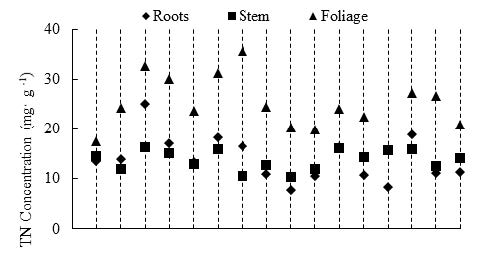
\includegraphics[width=\textwidth,height=0.3\textheight]{TN-p.jpg}}
	\subfigure{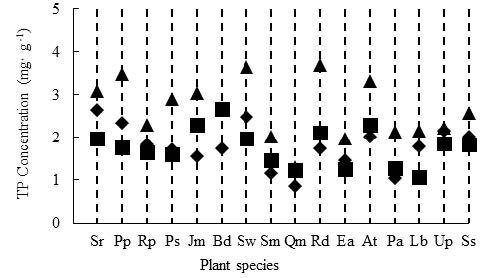
\includegraphics[width=\textwidth,height=0.3\textheight]{TP-p.jpg}}	
	%	\column{{0.01\textwidth}}
	\column{0.5\textwidth}
	\subfigure{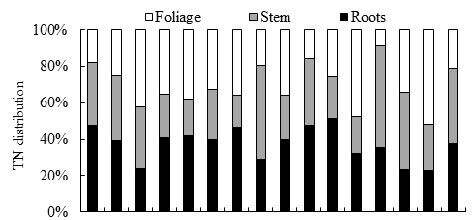
\includegraphics[width=\textwidth,height=0.3\textheight]{TN.jpg}}
	\subfigure{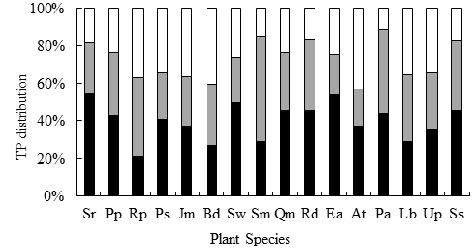
\includegraphics[width=\textwidth,height=0.3\textheight]{TP.jpg}}	
\end{columns}
\caption{Concentration and distribution of total nitrogen (TP) and total phosphorus (TP) in plants. \cite{yu2014biomass}}
%Syringa reticulate (Sr), Prunus padus (Pp), Robinia pseudoacacia (Rp), Pterocarya stenoptera (Ps), Juglans mandshuriea (Jm), Berberis dielsiana (Bd), Sambucus williamsii, Salix matsudana (Sm), Quercus mongolica (Qm), Rosa davurica (Rd), Euonymus alatus (Ea), Acer truncatum (At), Populus alba (Pa), Lespedeza bicolor (Lb), Ulmus pumila (Up) and Sorbaria sorbifolia (Ss). 

\end{figure}
\end{frame}

%Effects of stand structure on biodiversity and water-holding capacity
\begin{frame}{Effects of stand structure on species diversity and water-holding capacity}
\begin{table}
	\caption{Effects of stand structure on species diversity and water-holding capacity}
%	\begin{tabular}{@{}l@{}|@{}c@{}c@{}c@{}c@{}c@{}c@{}|@{}c@{}c@{}}
	\begin{tabular}{@{}l@{}|@{}cccccc@{}|@{}cc@{}}
		\toprule
		\multirow[c]{3}{4ex}{Treat-ment} & \multicolumn{6}{c}{Species number} & \multicolumn{2}{|c}{Water}\\
		&\multicolumn{3}{c}{First year} & \multicolumn{3}{c}{Second year}& \multicolumn{2}{|c}{storage ($t/hm^2$)}\\
		& Herb&Shrub & Tree &Herb&Shrub & Tree&Total& Non-capillary\\
		\midrule
		CK&3&7&14&3&7&15&1022&220\\
		Weak&3&7&15&3&8&16&1054&260\\
		Medium&4&8&16&4&8&18&1085&295\\
		Intense&4&8&18&5&10&20&1100&324\\
		\bottomrule
	\end{tabular}
\end{table}
\end{frame}
	\section{Application}

\begin{frame}{Demonstration projects}
There were three demonstration projects.  

\end{frame}

\begin{frame}{Take home message}
The study was successful. But it was expensive.

\end{frame}
	\begin{frame}[standout]
  Questions?
\end{frame}

\begin{frame}[standout]
Thanks for listening!
\end{frame}
	\appendix
\begin{frame}[shrink]{List of 68 plant species used in this study}
\tiny
\begin{columns}[T,onlytextwidth]
	\metroset{block=fill}
	\column{0.33\textwidth}
	\begin{block}{Tree}
		\begin{enumerate}
			\item \emph{Ulmus pumila} \item \emph{Syringa reticulate} \item \emph{Salix matsudana}
			\item \emph{Robinia pseudoacacia} \item \emph{Salix babylonica} \item \emph{Juglans mandshurica}
			\item \emph{Berberis dielsiana} \item \emph{Morus alba} \item \emph{Fraxinus mandschurica}
			\item \emph{Acer mono}	\item \emph{Fraxinus rhynchophylla}
			\item \emph{Prunus padus}	\item \emph{Ulmus davidiana} \item \emph{Armeniaca mandshurica}
			\item \emph{Pterocarya stenoptera}	\item \emph{Aralia elata} \item \emph{Quercus mongolica}
			\item \emph{Malus baccata}	\item \emph{Gleditsia microphylla } \item \emph{Crataegus pinnatifida}
			\item \emph{Acer negundo}	\item \emph{Celtis bungeana} \item \emph{Populus alba}
			\item \emph{Acer truncatum}	\item \emph{Betula allegheniensis} \item \emph{Tilia mandschurica}
			\item \emph{Salix koreensis}			
		\end{enumerate}	
	\end{block}
	
	\column{0.33\textwidth}
	\begin{alertblock}{Shrub}
		\begin{enumerate}			
			\item \emph{Lespedeza bicolor} \item \emph{Lonicera chrysantha} \item \emph{Sambucus williamsii}
			\item \emph{Sorbaria sorbifolia} \item \emph{Amorpha fruticose} \item \emph{Salix viminalis}
			\item \emph{Acer ginnala} \item \emph{Salix integra} \item \emph{Flueggea suffruticosa}
			\item \emph{Euonymus maackii}
			\item \emph{Lonicera maackii}	\item \emph{Philadelphus pekinensis} \item \emph{Cerasus tomentosa}
			\item \emph{Corylus heterophylla}	\item \emph{Actinidia arguta} \item \emph{Rosa davurica}
			\item \emph{Ampelopsis glandulosa}	\item \emph{Euonymus alatus} \item \emph{Rhamnus ussuriensis}
			\item \emph{Acanthopanax sessiliflorus}	\item \emph{Celastrus flagellaris}		
		\end{enumerate}	
	\end{alertblock}
	
	\column{0.33\textwidth}
	\begin{exampleblock}{Herb}		
		\begin{enumerate}			
			\item \emph{Phragmites australis} \item \emph{Artemisia capillaris} \item \emph{Sparganium stoloniferum}
			\item \emph{Impatiens noli-tangere} \item \emph{Polygonum persicaria} \item \emph{Iris pseudacorus}
			\item \emph{Acorus tatarinowii} \item \emph{Monochoria korsakowii} \item \emph{Iris sanguinea}
			\item \emph{Lythrum salicaria}
			\item \emph{Potentilla cryptotaeniae}	\item \emph{Polygonatum odoratum} \item \emph{Viola mandshurica}
			\item \emph{Corydalis bungeana}	\item \emph{Astilbe chinensis} \item \emph{Trrifolium repens}
			\item \emph{Arisaema peninsulae}	\item \emph{Ranunculus chinensis} \item \emph{Bidens biternata}
			\item \emph{Agrimonia pilosa}
		\end{enumerate}	
	\end{exampleblock}	
\end{columns}

\end{frame}

\begin{frame}[t,allowframebreaks]{References}
  \bibliography{bibliography}
%  \bibliographystyle{abbrv}
  \bibliographystyle{apalike}
\end{frame}
\end{document}
